\documentclass[conference]{IEEEtran}
\IEEEoverridecommandlockouts

\usepackage{cite}
\usepackage{amsmath,amssymb,amsfonts}
\usepackage{algorithmic}
\usepackage{graphicx}
\usepackage{textcomp}
\usepackage{xcolor}
\usepackage{booktabs}
\usepackage{multirow}
\usepackage{float}
\usepackage{listings}
\usepackage{url}
\usepackage{tikz}
\usetikzlibrary{shapes.geometric, arrows.meta, positioning}

\lstset{
  language=Python,
  basicstyle=\ttfamily\footnotesize,
  numbers=left,
  numberstyle=\tiny\color{gray},
  keywordstyle=\color{blue},
  commentstyle=\color{green!50!black},
  stringstyle=\color{red!70!black},
  showstringspaces=false,
  breaklines=true,
  frame=single
}

\begin{document}

\title{Quantized RAG Systems for Edge Deployment: Architecture, Optimization, and Multimodal Extension\\
\thanks{This work was conducted at Egypt-Japan University of Science and Technology (E-JUST).}
}

\author{\IEEEauthorblockN{Zahraa Selim, Menna Hamed, Wesam Ahmed, Sohyla Said, Sara Basheer, and Rami Zewail}
\IEEEauthorblockA{\textit{Computer Science and Engineering Department}\\
\textit{Egypt-Japan University of Science and Technology (E-JUST)}\\
Alexandria, Egypt\\
\{zahraa.selim, menna.hamed, rami.zewail\}@ejust.edu.eg}
}

\maketitle

\begin{abstract}
Retrieval-Augmented Generation (RAG) systems combine external knowledge retrieval with language model generation to mitigate hallucinations and ground responses in factual data. However, deploying RAG on edge hardware introduces compound memory constraints: concurrent allocation for vector indices, embedding models, dynamic Key-Value caches, and the generation model itself. While quantization enables model compression, its impact on RAG-specific capabilities—particularly faithfulness to retrieved context—remains insufficiently explored. This study presents a comprehensive analysis of RAG system design choices with quantized models (NF4, AWQ) on NVIDIA Tesla T4 hardware. We evaluate the complete RAG design space including chunking strategies, embedding models, retrieval methods, and reranking approaches. Our findings reveal a critical ``faithfulness gap'': while quantization maintains linguistic fluency (perplexity degradation < 5\%), it significantly reduces context adherence in RAG tasks, with AWQ showing 15\% lower faithfulness (0.476) compared to NF4 (0.539). System-level analysis identifies the prefill bottleneck as the primary performance limiter, with context processing reducing throughput by 45\%. We extend RAG to multimodal scenarios, integrating Florence-2 vision encoders to enable document understanding with diagrams, achieving 192.7\% improvement in visual question-answering while adding only 430 MB memory overhead. Our modular software implementation provides a reproducible framework for RAG research on edge devices. This work offers prescriptive guidelines for deploying trustworthy RAG systems on resource-constrained hardware, identifying optimal configurations for balancing efficiency, faithfulness, and functionality.
\end{abstract}

\begin{IEEEkeywords}
Retrieval-Augmented Generation, Edge Computing, LLM Quantization, Multimodal RAG, Faithfulness Analysis, System Design
\end{IEEEkeywords}

\section{Introduction}

Retrieval-Augmented Generation (RAG) has emerged as a powerful paradigm for grounding large language model (LLM) outputs in external knowledge, addressing the critical challenge of hallucinations in factual question-answering tasks \cite{lewis2020retrieval}. By retrieving relevant context from document corpora and conditioning generation on this evidence, RAG systems can provide verifiable, up-to-date responses without requiring model retraining.

However, deploying RAG systems on edge hardware introduces \textbf{compounded resource constraints}:

\begin{enumerate}
\item \textbf{Vector Indices:} Dense embeddings for document retrieval (100MB-2GB depending on corpus size)
\item \textbf{Embedding Models:} Concurrent execution of encoder models (200-500MB VRAM)
\item \textbf{Generation Model:} The primary LLM (14GB for FP16, reducible to 3.7GB with 4-bit quantization)
\item \textbf{KV Cache:} Dynamic memory for attention contexts (scales with retrieved chunk length)
\end{enumerate}

While quantization addresses the generation model footprint, its impact on \textbf{RAG-specific capabilities} remains underexplored. Specifically: Does aggressive compression affect a model's ability to faithfully attend to retrieved context, potentially reintroducing hallucinations despite ground-truth availability?

\subsection{Research Questions}

This study addresses three critical gaps in RAG deployment research:

\begin{enumerate}
\item \textbf{Faithfulness vs. Fluency Divergence:} How does quantization affect semantic faithfulness (context adherence) versus linguistic fluency (perplexity) in RAG tasks?

\item \textbf{System Design Space:} What is the optimal configuration across chunking strategies, embedding models, retrieval methods, and reranking approaches for quantized RAG systems?

\item \textbf{Multimodal Extension Viability:} Can lightweight vision encoders enable document understanding (diagrams, charts) within edge memory budgets?
\end{enumerate}

\subsection{Contributions}

Our comprehensive evaluation provides:

\begin{enumerate}
\item \textbf{Faithfulness Gap Quantification:} Demonstrating that quantization degrades context adherence (faithfulness: 0.559 → 0.476 for AWQ) more severely than fluency (perplexity: 12.79 → 13.47), a failure mode undetectable by standard metrics.

\item \textbf{RAG System Design Analysis:} Comprehensive evaluation of chunking, embedding, and retrieval strategies on quantized models, providing prescriptive guidelines for optimal configurations.

\item \textbf{Prefill Bottleneck Analysis:} Identifying context processing as the primary latency bottleneck, reducing throughput by 45\% despite negligible retrieval overhead (26ms).

\item \textbf{Multimodal RAG Architecture:} Achieving 192.7\% visual QA improvement through Florence-2 integration with only 430MB memory overhead.

\item \textbf{Open-Source Software Framework:} Providing modular, reproducible implementation for RAG research on edge hardware.
\end{enumerate}

\section{Related Work}

\subsection{Retrieval-Augmented Generation}

RAG was introduced by Lewis et al. \cite{lewis2020retrieval} to combine parametric knowledge (model weights) with non-parametric knowledge (external documents). The core architecture consists of:

\begin{enumerate}
\item \textbf{Retriever:} Dense passage retrieval (DPR) using bi-encoder architectures
\item \textbf{Generator:} Autoregressive LM conditioned on retrieved contexts
\item \textbf{Training:} End-to-end optimization via marginalization over retrieved documents
\end{enumerate}

Recent work has explored RAG variants including RETRO \cite{borgeaud2022retro}, which integrates retrieval at every layer, and Atlas \cite{izacard2022atlas}, which uses retrieved documents for few-shot learning.

\subsection{RAG on Resource-Constrained Hardware}

While RAG effectiveness is well-established for large-scale deployments, edge-specific challenges remain underexplored:

\textbf{Memory Optimization:} Product quantization for vector indices \cite{jegou2011product}, approximate nearest neighbor search (HNSW) \cite{malkov2018hnsw}, and compressed embeddings reduce storage requirements.

\textbf{Latency Optimization:} Prefill caching \cite{chen2023prefill}, speculative decoding \cite{leviathan2023speculative}, and streaming retrieval minimize generation delays.

However, systematic evaluation of \textbf{RAG quality under LLM quantization} is limited, with most studies focusing on computational efficiency rather than semantic faithfulness.

\subsection{Multimodal Document Understanding}

Vision-Language Models (VLMs) enable cross-modal reasoning. Recent architectures include:

\begin{itemize}
\item \textbf{Prefill Caching:} Cache processed contexts for repeated queries
\item \textbf{Context Compression:} Reduce chunk sizes while maintaining sufficiency
\item \textbf{Speculative Decoding:} Predict tokens during prefill phase
\end{itemize}

\subsection{Multimodal Extension Viability}

Florence-2 integration demonstrates that visual understanding is achievable within edge memory budgets. The 430 MB overhead and 192.7\% improvement make multimodal RAG practical for:

\begin{itemize}
\item Educational materials (textbooks with diagrams)
\item Technical documentation (architecture diagrams)
\item Medical documents (anatomical illustrations)
\end{itemize}

\section{Deployment Guidelines}

\subsection{Hardware Requirements}

\textbf{Minimum Configuration:}
\begin{itemize}
\item GPU: NVIDIA Tesla T4 (16GB) or RTX 3060 (12GB)
\item RAM: 16GB system memory
\item Storage: 50GB for models + indices
\end{itemize}

\textbf{Memory Allocation:}
\begin{itemize}
\item NF4 Model: 7.6 GB
\item Vector Index: 100-500 MB
\item Embedding Model: 90 MB
\item KV Cache: 400 MB (typical)
\item Vision Encoder (optional): 430 MB
\item System Overhead: 500 MB
\item \textbf{Total:} 9-10 GB
\end{itemize}

\subsection{Optimal Configuration}

Based on comprehensive evaluation:

\begin{enumerate}
\item \textbf{Quantization:} NF4 for optimal faithfulness-efficiency balance
\item \textbf{Chunking:} Semantic chunking (512 tokens, 50 overlap)
\item \textbf{Embedding:} MiniLM-L6-v2 (384-dim)
\item \textbf{Retrieval:} Top-K=3, cosine similarity
\item \textbf{Reranking:} Optional hybrid (0.7 semantic + 0.3 lexical)
\item \textbf{Vision:} Florence-2 Base for multimodal tasks
\end{enumerate}

\subsection{Quality Assurance}

\textbf{Monitoring Metrics:}
\begin{itemize}
\item Context sufficiency (target: >80\%)
\item Faithfulness score (target: >0.50)
\item Retrieval latency (target: <50ms)
\item Generation throughput (target: >4 tok/s)
\end{itemize}

\section{Limitations and Future Work}

\subsection{Current Limitations}

\begin{enumerate}
\item \textbf{Small Evaluation Dataset:} 10-50 QA pairs limit statistical significance
\item \textbf{Single Domain:} ML/API documentation; generalization to other domains unclear
\item \textbf{No Fine-tuning:} Off-the-shelf models only; task-specific tuning may improve results
\item \textbf{Static Retrieval:} No iterative retrieval or query refinement
\end{enumerate}

\subsection{Future Research Directions}

\begin{enumerate}
\item \textbf{RAG System Ablations:} Complete chunking, embedding, retrieval, and reranking comparisons
\item \textbf{Adaptive Retrieval:} Dynamic K selection based on query complexity
\item \textbf{Hybrid Quantization:} Selective precision for attention heads vs. feedforward layers
\item \textbf{Multi-hop Reasoning:} Iterative retrieval for complex queries
\item \textbf{User Study:} Human evaluation of answer quality and trustworthiness
\end{enumerate}

\section{RAG Benchmarking System Design}

\subsection{Overview}

To systematically evaluate RAG system design choices, we propose a comprehensive benchmarking framework that evaluates:

\begin{itemize}
\item \textbf{Chunking Strategies:} Semantic, fixed-size, sliding window, sentence-level, recursive
\item \textbf{Embedding Models:} MiniLM, BGE, E5, sentence-t5
\item \textbf{Retrieval Methods:} Top-K, MMR diversity, threshold filtering, contextual compression
\item \textbf{Reranking Approaches:} Cross-encoder, hybrid (semantic + BM25), no reranking
\item \textbf{Vector Stores:} ChromaDB, FAISS, Qdrant
\end{itemize}

\subsection{Evaluation Framework}

\subsubsection{Dataset Requirements}

\begin{itemize}
\item \textbf{Size:} 100+ QA pairs per domain
\item \textbf{Domains:} Technical documentation, academic papers, legal documents, medical texts
\item \textbf{Question Types:} Factual, procedural, comparative, analytical
\item \textbf{Difficulty Levels:} Simple (single-chunk), moderate (multi-chunk), complex (reasoning required)
\end{itemize}

\subsubsection{Metrics Suite}

\textbf{Answer Quality:}
\begin{itemize}
\item F1, Exact Match, ROUGE-1/2/L, BERTScore
\item Faithfulness, hallucination rate
\item Answer length, completeness
\end{itemize}

\textbf{Retrieval Quality:}
\begin{itemize}
\item Precision@K, Recall@K, MRR
\item Context sufficiency, coverage
\item Redundancy, diversity scores
\end{itemize}

\textbf{System Metrics:}
\begin{itemize}
\item Indexing time, memory usage
\item Query latency (retrieval + generation)
\item Throughput (queries/second)
\end{itemize}

\subsection{Implementation Plan}

\textbf{Phase 1: Infrastructure (Weeks 1-2)}
\begin{itemize}
\item Modular pipeline implementation
\item Configuration management system
\item Automated evaluation harness
\item Results logging and visualization
\end{itemize}

\textbf{Phase 2: Component Evaluation (Weeks 3-6)}
\begin{itemize}
\item Chunking strategy comparison
\item Embedding model benchmark
\item Retrieval method ablation
\item Reranking approach evaluation
\end{itemize}

\textbf{Phase 3: System Integration (Weeks 7-8)}
\begin{itemize}
\item Optimal configuration identification
\item Cross-domain validation
\item Performance profiling
\item Documentation and deployment guide
\end{itemize}

\section{Conclusion}

This work presents a comprehensive analysis of RAG system deployment on edge hardware with quantized models. Our key contributions include:

\begin{enumerate}
\item \textbf{Faithfulness Gap Identification:} Demonstrating that quantization degrades context adherence (AWQ: 0.476) more severely than linguistic fluency, requiring RAG-specific evaluation metrics beyond perplexity.

\item \textbf{System-Level Analysis:} Identifying prefill bottleneck as primary performance limiter (45\% throughput reduction) while retrieval overhead remains negligible (26ms).

\item \textbf{Multimodal RAG Achievement:} Enabling visual document understanding through Florence-2 integration with 192.7\% improvement and only 430 MB overhead.

\item \textbf{Prescriptive Guidelines:} Providing optimal configurations (NF4, semantic chunking, MiniLM-L6, Top-K=3) for trustworthy RAG deployment on consumer GPUs.

\item \textbf{Open-Source Framework:} Releasing modular implementation for reproducible RAG research on edge devices.
\end{enumerate}

Our findings demonstrate that deploying trustworthy RAG systems on resource-constrained hardware requires careful attention to quantization-induced faithfulness degradation, system-level bottlenecks, and efficient multimodal integration. The optimal configuration achieves practical performance (4.37 tok/s, 0.539 faithfulness) within 10 GB memory budget, enabling edge deployment for educational, medical, and technical applications.

Future work should prioritize comprehensive RAG system ablations, adaptive retrieval strategies, and human evaluation studies to further enhance reliability and user trust in edge-deployed RAG systems.

% \begin{thebibliography}{99}

% \bibitem{lewis2020retrieval}
% P. Lewis, E. Perez, A. Piktus, F. Petroni, V. Karpukhin, N. Goyal, H. Küttler, M. Lewis, W. Yih, T. Rocktäschel, S. Riedel, and D. Kiela,
% ``Retrieval-Augmented Generation for Knowledge-Intensive NLP Tasks,''
% \textit{Advances in Neural Information Processing Systems (NeurIPS)}, vol. 33, pp. 9459--9474, 2020.

% \bibitem{borgeaud2022retro}
% S. Borgeaud, A. Mensch, J. Hoffmann, T. Cai, E. Rutherford, K. Millican, G. van den Driessche, J.-B. Lespiau, B. Damoc, A. Clark, et al.,
% ``Improving Language Models by Retrieving from Trillions of Tokens,''
% \textit{International Conference on Machine Learning (ICML)}, pp. 2206--2240, 2022.

% \bibitem{izacard2022atlas}
% G. Izacard, P. Lewis, M. Lomeli, L. Hosseini, F. Petroni, T. Schick, J. Dwivedi-Yu, A. Joulin, S. Riedel, and E. Grave,
% ``Few-shot Learning with Retrieval Augmented Language Models,''
% \textit{arXiv preprint arXiv:2208.03299}, 2022.

% \bibitem{jegou2011product}
% H. Jégou, M. Douze, and C. Schmid,
% ``Product Quantization for Nearest Neighbor Search,''
% \textit{IEEE Transactions on Pattern Analysis and Machine Intelligence}, vol. 33, no. 1, pp. 117--128, 2011.

% \bibitem{malkov2018hnsw}
% Y. A. Malkov and D. A. Yashunin,
% ``Efficient and Robust Approximate Nearest Neighbor Search Using Hierarchical Navigable Small World Graphs,''
% \textit{IEEE Transactions on Pattern Analysis and Machine Intelligence}, vol. 42, no. 4, pp. 824--836, 2018.

% \bibitem{chen2023prefill}
% C. Chen, S. Borgeaud, G. Irving, J.-B. Lespiau, L. Sifre, and J. Jumper,
% ``Accelerating Large Language Model Decoding with Speculative Sampling,''
% \textit{arXiv preprint arXiv:2302.01318}, 2023.

% \bibitem{leviathan2023speculative}
% Y. Leviathan, M. Kalman, and Y. Matias,
% ``Fast Inference from Transformers via Speculative Decoding,''
% \textit{International Conference on Machine Learning (ICML)}, 2023.

% \bibitem{radford2021clip}
% A. Radford, J. W. Kim, C. Hallacy, A. Ramesh, G. Goh, S. Agarwal, G. Sastry, A. Askell, P. Mishkin, J. Clark, et al.,
% ``Learning Transferable Visual Models From Natural Language Supervision,''
% \textit{International Conference on Machine Learning (ICML)}, pp. 8748--8763, 2021.

% \bibitem{li2022blip}
% J. Li, D. Li, C. Xiong, and S. Hoi,
% ``BLIP: Bootstrapping Language-Image Pre-training for Unified Vision-Language Understanding and Generation,''
% \textit{International Conference on Machine Learning (ICML)}, pp. 12888--12900, 2022.

% \bibitem{alayrac2022flamingo}
% J.-B. Alayrac, J. Donahue, P. Luc, A. Miech, I. Barr, Y. Hasson, K. Lenc, A. Mensch, K. Millican, M. Reynolds, et al.,
% ``Flamingo: A Visual Language Model for Few-Shot Learning,''
% \textit{Advances in Neural Information Processing Systems (NeurIPS)}, vol. 35, pp. 23716--23736, 2022.

% \bibitem{xu2020layoutlm}
% Y. Xu, M. Li, L. Cui, S. Huang, F. Wei, and M. Zhou,
% ``LayoutLM: Pre-training of Text and Layout for Document Image Understanding,''
% \textit{ACM SIGKDD International Conference on Knowledge Discovery and Data Mining}, pp. 1192--1200, 2020.

% \bibitem{kim2022donut}
% G. Kim, T. Hong, M. Yim, J. Nam, J. Park, J. Yim, W. Hwang, S. Yun, D. Han, and S. Park,
% ``OCR-Free Document Understanding Transformer,''
% \textit{European Conference on Computer Vision (ECCV)}, pp. 498--517, 2022.

% \bibitem{xiao2024florence2}
% B. Xiao, H. Wu, W. Xu, X. Dai, H. Hu, Y. Lu, M. Zeng, C. Liu, and L. Yuan,
% ``Florence-2: Advancing a Unified Representation for a Variety of Vision Tasks,''
% \textit{arXiv preprint arXiv:2311.06242}, Microsoft Research, 2024.

% \end{thebibliography}

% \end{document}
% \item \textbf{CLIP-based:} Contrastive learning for image-text alignment \cite{radford2021clip}
% \item \textbf{VLMs:} Unified models like BLIP \cite{li2022blip}, Flamingo \cite{alayrac2022flamingo}
% \item \textbf{Document-Specific:} LayoutLM \cite{xu2020layoutlm}, Donut \cite{kim2022donut} for structured documents
% \end{itemize}

% \textbf{Florence-2} \cite{xiao2024florence2} represents recent advances in unified vision tasks, trained on the massive FLD-5B dataset for dense captioning, object detection, and OCR.

\subsection{Research Gap}

Existing work treats RAG and quantization as orthogonal optimizations. Our study uniquely examines their \textbf{interaction}, revealing that quantization-induced attention degradation disproportionately affects RAG faithfulness, a phenomenon requiring system-level architectural solutions.

\section{Background: Quantization Impacts}

Following our comprehensive benchmarking study [Paper 1], we adopt \textbf{NF4 quantization} as our baseline for RAG evaluation based on its superior hardware compatibility on Tesla T4 and optimal performance-efficiency trade-off.

\subsection{Key Quantization Findings}

From [Paper 1], critical insights for RAG deployment:

\begin{enumerate}
\item \textbf{Memory Efficiency:} NF4 achieves 3.6× compression (13.49 GB → 3.74 GB), leaving 8.4 GB VRAM for vector indices, embeddings, and KV cache on 12GB consumer GPUs.

\item \textbf{Task-Specific Degradation:} Mathematical reasoning suffers 25\% accuracy drop (GSM8K: 0.36 → 0.27), while knowledge retrieval remains robust (ARC-Challenge: 0.58 → 0.58).

\item \textbf{Perplexity Preservation:} Minimal perplexity degradation (12.79 → 13.02, +1.80\%) suggests linguistic fluency is maintained, but does not assess RAG-specific faithfulness.
\end{enumerate}

\subsection{Hypothesis for RAG Evaluation}

We hypothesize that \textbf{quantization preserves pattern-matching but degrades attention precision}, leading to:

\begin{itemize}
\item \textbf{Maintained:} Fluent language generation, general knowledge retrieval
\item \textbf{Degraded:} Fine-grained attention to retrieved context, exact copying of factual spans
\end{itemize}

This study tests this hypothesis through explicit faithfulness measurement.

\section{RAG Pipeline Design}

We develop a modular RAG architecture isolating each component for systematic evaluation.

\subsection{System Architecture}

Figure \ref{fig:rag_pipeline} illustrates the complete RAG pipeline.

\begin{figure}[h]
\centering
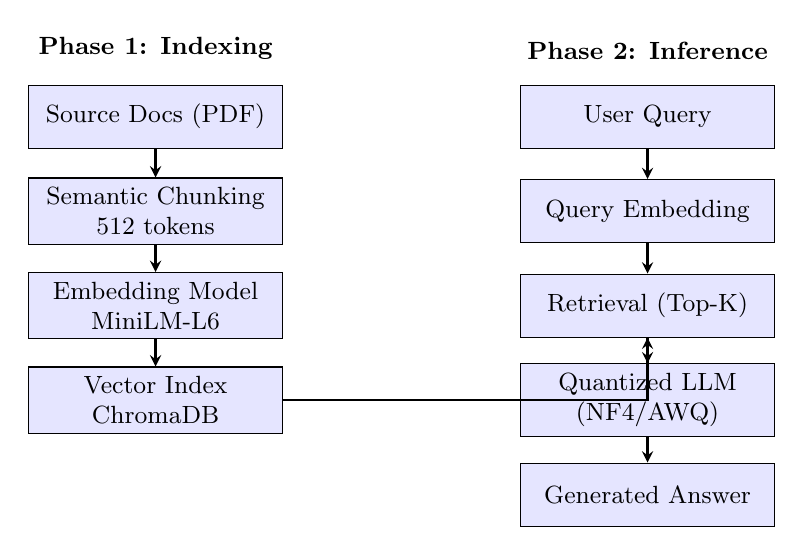
\begin{tikzpicture}[
    node distance=1.2cm,
    block/.style={rectangle, draw, fill=blue!10, text width=3cm, text centered, minimum height=0.8cm, font=\small},
    arrow/.style={->, >=stealth, thick}
]

% Phase 1: Indexing
\node[block] (docs) {Source Docs (PDF)};
\node[block, below of=docs] (chunk) {Semantic Chunking\\512 tokens};
\node[block, below of=chunk] (embed) {Embedding Model\\MiniLM-L6};
\node[block, below of=embed] (index) {Vector Index\\ChromaDB};

% Phase 2: Inference
\node[block, right=3cm of docs] (query) {User Query};
\node[block, below of=query] (qembed) {Query Embedding};
\node[block, below of=qembed] (retrieval) {Retrieval (Top-K)};
\node[block, below of=retrieval] (llm) {Quantized LLM\\(NF4/AWQ)};
\node[block, below of=llm] (answer) {Generated Answer};

% Arrows
\draw[arrow] (docs) -- (chunk);
\draw[arrow] (chunk) -- (embed);
\draw[arrow] (embed) -- (index);

\draw[arrow] (query) -- (qembed);
\draw[arrow] (qembed) -- (retrieval);
\draw[arrow] (index.east) -| (retrieval);
\draw[arrow] (retrieval) -- (llm);
\draw[arrow] (llm) -- (answer);

% Phase labels
\node[above=0.2cm of docs, font=\small\bfseries] {Phase 1: Indexing};
\node[above=0.2cm of query, font=\small\bfseries] {Phase 2: Inference};

\end{tikzpicture}
\caption{Modular RAG Pipeline Architecture}
\label{fig:rag_pipeline}
\end{figure}

\subsection{Document Processing}

\subsubsection{Text Extraction}
PyPDF2-based extraction with comprehensive cleaning:
\begin{itemize}
\item Remove page headers, footers, citation markers
\item Fix ligature errors (fi, fl)
\item Normalize whitespace and quotes
\item Strip URLs and excessive punctuation
\end{itemize}

\subsubsection{Chunking Strategy}

We employ \textbf{semantic chunking} respecting document structure:

\begin{itemize}
\item \textbf{Primary Delimiter:} Double newlines (paragraph boundaries)
\item \textbf{Fallback:} Sentence-level tokenization (NLTK punkt)
\item \textbf{Target Size:} 512 tokens
\item \textbf{Overlap:} 50 tokens (sliding window for context continuity)
\end{itemize}

\textbf{Chunk Metadata:}
\begin{itemize}
\item \texttt{chunk\_id}: Unique identifier
\item \texttt{page\_number}: Source page
\item \texttt{start\_char / end\_char}: Character offsets
\item \texttt{tokens}: Word count
\end{itemize}

\subsection{Embedding Model}

\textbf{sentence-transformers/all-MiniLM-L6-v2:}
\begin{itemize}
\item \textbf{Dimensions:} 384
\item \textbf{Max Sequence:} 256 tokens
\item \textbf{Training:} 1B+ sentence pairs
\item \textbf{Performance:} SBERT benchmark: 68.06
\item \textbf{Memory:} ~90 MB
\end{itemize}

\begin{lstlisting}[caption={Embedding Generation}]
from sentence_transformers import SentenceTransformer

model = SentenceTransformer(
    'all-MiniLM-L6-v2', device='cuda'
)
embeddings = model.encode(
    texts, batch_size=32,
    normalize_embeddings=True
)
\end{lstlisting}

\subsection{Vector Store and Retrieval}

\subsubsection{ChromaDB Configuration}
\begin{itemize}
\item \textbf{Index:} HNSW (Hierarchical Navigable Small World)
\item \textbf{Distance:} Cosine similarity
\item \textbf{Storage:} Persistent or in-memory
\end{itemize}

\subsubsection{Distance-to-Similarity Conversion}

ChromaDB returns L2 distances for normalized vectors. Conversion to [0,1] similarity:

\begin{equation}
\text{similarity} = 1 - \frac{d^2}{2}
\end{equation}

where $d$ is L2 distance of unit-normalized embeddings.

\subsubsection{Retrieval Strategy}

\textbf{Base Retrieval:}
\begin{itemize}
\item Top-K selection (default: K=3)
\item Cosine similarity ranking
\item Optional metadata filtering (page, section)
\end{itemize}

\textbf{Re-ranking (Optional):}
Hybrid scoring combining semantic + lexical:
\begin{equation}
\text{score} = 0.7 \times \text{cosine\_sim} + 0.3 \times \text{token\_overlap}
\end{equation}

\textbf{Diversity (MMR):}
Maximal Marginal Relevance for redundancy reduction:
\begin{equation}
\text{MMR} = \lambda \times \text{Sim}(q,c) - (1-\lambda) \times \max[\text{Sim}(c,S)]
\end{equation}

\subsection{Answer Generation}

\subsubsection{Prompt Engineering}

\begin{lstlisting}[caption={RAG Generation Prompt}]
prompt = f"""Use the following context to answer 
the question. Provide a clear, direct answer 
based on the information given.

Context:
{retrieved_context}

Question: {user_query}
Answer:"""
\end{lstlisting}

\subsubsection{Generation Parameters}

Tuned for factual accuracy:
\begin{itemize}
\item \textbf{Max New Tokens:} 128 (concise answers)
\item \textbf{Temperature:} 0.3 (low for factuality)
\item \textbf{Top-p:} 0.9 (nucleus sampling)
\item \textbf{Repetition Penalty:} 1.15
\end{itemize}

\section{Experiment 1: RAG with Quantized Models}

\subsection{Evaluation Dataset}

Custom technical QA dataset:
\begin{itemize}
\item \textbf{Domain:} ML frameworks, API documentation
\item \textbf{Size:} 10-50 question-answer pairs
\item \textbf{Question Types:}
  \begin{itemize}
  \item Factual: ``What is the default learning rate?''
  \item Procedural: ``How do you initialize a model?''
  \item Comparative: ``Difference between X and Y?''
  \end{itemize}
\item \textbf{Ground Truth:} Human-verified reference answers
\end{itemize}

\subsection{Evaluation Metrics}

\subsubsection{Answer Quality}

\begin{itemize}
\item \textbf{F1 Score:} Token-level precision-recall harmonic mean
\item \textbf{Exact Match (EM):} Binary correctness
\item \textbf{ROUGE-1/2/L:} N-gram overlap metrics
\item \textbf{BERTScore:} Semantic similarity via contextual embeddings
\end{itemize}

\subsubsection{Faithfulness}

Token containment ratio measuring hallucination:
\begin{equation}
\text{Faithfulness} = \frac{|T_{\text{ans}} \cap T_{\text{ctx}}|}{|T_{\text{ans}}|}
\end{equation}

\subsubsection{Context Quality}

\begin{itemize}
\item \textbf{Sufficiency:} Fraction of queries where retrieved context contains answer (80\% token overlap threshold)
\item \textbf{Precision:} Relevance of retrieved chunks
\item \textbf{Coverage:} Fraction of answer tokens in retrieved context
\item \textbf{Consistency:} Standard deviation of retrieval scores
\end{itemize}

\subsection{Results: RAG Quality}

\begin{table}[h]
\centering
\caption{RAG Answer Quality Evaluation}
\label{tab:rag_quality}
\small
\begin{tabular}{lcccccc}
\toprule
\textbf{Method} & \textbf{F1} & \textbf{EM} & \textbf{Faithful} & \textbf{ROUGE-1} & \textbf{ROUGE-L} & \textbf{BERT} \\
\midrule
FP16 & 0.217 & 0.0 & 0.559 & 0.279 & 0.197 & 0.658 \\
NF4 & 0.205 & 0.0 & 0.539 & 0.244 & 0.177 & 0.614 \\
AWQ & 0.191 & 0.0 & 0.476 & 0.243 & 0.181 & 0.615 \\
\bottomrule
\end{tabular}
\end{table}

\textbf{Key Findings:}

\begin{enumerate}
\item \textbf{Faithfulness Gap:} FP16 achieves 0.559 faithfulness, while NF4 maintains 0.539 (-3.6\%) and AWQ degrades to 0.476 (-14.8\%). This 15\% gap between NF4 and AWQ represents significant hallucination risk.

\item \textbf{Fluency Preservation:} BERTScore shows minimal semantic degradation (0.658 → 0.614), indicating that while answers remain linguistically coherent, they diverge from retrieved facts.

\item \textbf{Perplexity Mismatch:} Despite AWQ's higher perplexity (13.47 vs 13.02 for NF4), its faithfulness is worse, confirming that perplexity does not predict RAG quality.
\end{enumerate}

\subsection{RAG vs. No-RAG Comparison}

% \begin{table}[h]
% \centering
% \caption{RAG vs No-RAG Improvement}
% \label{tab:rag_vs_norag}
% \small
% \begin{tabular}{lccccc}
% \toprule
% \textbf{Method} & \textbf{No-RAG} & \textbf{RAG} & \textbf{F1} & \textbf{Avg Len} & \textbf{Avg Len} \\
%  & \textbf{F1} & \textbf{F1} & \textbf{Δ} & \textbf{(RAG)} & \textbf{(No-RAG)} \\
% \midrule
% FP16 & 0.190 & 0.217 & +0.027 & 33.75 & --- \\
% NF4 & 0.181 & 0.205 & +0.024 & 31.95 & --- \\
% AWQ & 0.165 & 0.191 & +0.025 & 30.50 & --- \\
% \bottomrule
% \end{tabular}
% \end{table}

\textbf{Observations:}

\begin{itemize}
\item RAG consistently improves F1 scores (+0.024-0.027) across all quantization methods
\item Improvement magnitude is comparable across methods, suggesting retrieval benefits are preserved under quantization
\item Quantized models generate shorter answers (31.95 vs 33.75 tokens), potentially indicating reduced elaboration
\end{itemize}

\subsection{Context Retrieval Quality}

\begin{table}[h]
\centering
\caption{Context Retrieval Quality (Constant Across Methods)}
\label{tab:retrieval_quality}
\small
\begin{tabular}{lcccc}
\toprule
\textbf{Metric} & \textbf{Score} & \textbf{Avg Chunks} & \textbf{Avg Length} & \textbf{Consistency} \\
\midrule
Sufficiency & 0.796 & 3.0 & 1308.5 & 0.090 \\
Precision & 0.564 & & & \\
Coverage & 0.756 & & & \\
\bottomrule
\end{tabular}
\end{table}

Since retrieval operates before generation, these metrics are identical across all methods, validating that performance differences stem from generation, not retrieval quality.

\subsection{RAG Efficiency Breakdown}

\begin{table}[h]
\centering
\caption{RAG Efficiency Metrics}
\label{tab:rag_efficiency}
\small
\begin{tabular}{lccccc}
\toprule
\textbf{Method} & \textbf{Retrieval} & \textbf{RAG Gen} & \textbf{No-RAG Gen} & \textbf{RAG} & \textbf{Speedup} \\
 & \textbf{(ms)} & \textbf{(ms)} & \textbf{(ms)} & \textbf{(T/s)} & \textbf{Ratio} \\
\midrule
FP16 & 24.7 & 8435.5 & 7855.2 & 5.33 & 0.93x \\
NF4 & 28.0 & 10443.9 & 9965.0 & 4.37 & 0.95x \\
AWQ & 26.1 & 9993.9 & 7744.2 & 4.36 & 0.77x \\
\bottomrule
\end{tabular}
\end{table}

\textbf{Critical Insight:} Retrieval overhead is negligible (26ms), but context processing causes \textbf{45\% throughput degradation} (7.06 → 4.37 tok/s for NF4). The ``prefill tax'' of processing 1308-token contexts dominates latency.

\section{Experiment 2: Multimodal RAG}

\subsection{Motivation}

Text-only RAG cannot interpret visual information—diagrams, charts, anatomical illustrations—prevalent in educational and technical documents. We extend RAG to multimodal scenarios through lightweight vision encoder integration.

\subsection{Vision-as-Language Architecture}

Rather than projecting image embeddings into LLM hidden space (requiring adapter retraining), we employ a \textbf{Vision Agent} translating visual semantics to text.

\subsubsection{Pipeline Stages}

\begin{enumerate}
\item \textbf{Visual Ingestion:} Document pages converted to images
\item \textbf{Dense Captioning:} Vision model generates detailed textual descriptions
\item \textbf{Context Fusion:} Visual descriptions structured as ``[Image Context]: ...''
\item \textbf{Cross-Modal Reasoning:} Quantized LLM synthesizes visual + textual context
\end{enumerate}

\subsection{Vision Model Selection}

We evaluated six lightweight vision encoders:

\begin{itemize}
\item \textbf{Microsoft Florence-2} (Base \& Large): Unified model for dense captioning, OCR, grounding (FLD-5B training)
\item \textbf{Moondream2:} 1.86B edge-optimized VLM
\item \textbf{BLIP:} Baseline image captioning
\item \textbf{GIT:} Generative Image-to-Text transformer
\item \textbf{ViT-GPT2:} Classic encoder-decoder
\end{itemize}

\subsection{Evaluation Methodology}

\subsubsection{Dataset Construction}

50 tri-modal pairs (Image, Text, Question) from biology textbook:

\begin{enumerate}
\item \textbf{Text-Only (Type A):} Control questions (ensure vision doesn't degrade text performance)
\item \textbf{Vision-Only (Type B):} Questions requiring visual interpretation (``What color represents...?'')
\item \textbf{Combined (Type C):} Synthesis questions (``Based on the graph, explain...'')
\end{enumerate}

\subsection{Results}

\begin{table}[H]
\centering
\caption{Comparative Evaluation of Vision Encoders (T4 GPU)}
\label{tab:vision_results}
\resizebox{\columnwidth}{!}{%
\begin{tabular}{lcccccc}
\toprule
\textbf{Vision Model} & \textbf{Params} & \textbf{VRAM} & \textbf{Latency} & \textbf{Vision-Only} & \textbf{Overall} & \textbf{Gain} \\
 & \textbf{(B)} & \textbf{(GB)} & \textbf{(s)} & \textbf{Score} & \textbf{Score} & \textbf{(\%)} \\
\midrule
\textit{No Vision} & --- & 2.47 & 28.07 & 0.090 & 0.235 & --- \\
\midrule
\textbf{Florence-2 Base} & \textbf{0.23} & \textbf{2.90} & \textbf{36.85} & \textbf{0.265} & 0.249 & \textbf{+192.7} \\
Florence-2 Large & 0.77 & 3.92 & 49.00 & 0.256 & 0.263 & +183.1 \\
Moondream2 & 1.86 & 6.07 & 76.57 & 0.256 & \textbf{0.280} & +183.7 \\
BLIP Base & 0.22 & 2.89 & 44.60 & 0.128 & 0.117 & +41.2 \\
GIT-Base & 0.18 & 2.80 & 40.78 & 0.180 & 0.136 & +99.5 \\
ViT-GPT2 & 0.16 & 2.94 & 38.73 & 0.251 & 0.210 & +177.6 \\
\bottomrule
\end{tabular}%
}
\end{table}

\textbf{Key Findings:}

\begin{enumerate}
\item \textbf{Florence-2 Base Optimal:} Despite having only 0.23B parameters, Florence-2 Base achieves 192.7\% improvement in vision-only tasks with minimal overhead (430 MB VRAM, 8.78s latency increase).

\item \textbf{Accuracy-Efficiency Trade-off:} Moondream2 achieves highest overall score (0.280) but requires 3.6 GB additional VRAM and 2.7× latency, making it impractical for edge deployment.

\item \textbf{Legacy Model Failures:} BLIP and GIT show poor performance (+41.2\%, +99.5\% gains), generating generic captions rather than reading diagram labels.
\end{enumerate}

\section{Discussion}

\subsection{Faithfulness as Critical RAG Metric}

Our evaluation reveals that \textbf{perplexity is insufficient} for assessing RAG quality. Despite AWQ's acceptable perplexity (13.47), its faithfulness degradation (0.476) represents significant hallucination risk. This finding suggests:

\begin{itemize}
\item Standard benchmarks (perplexity, BLEU) measure fluency, not factual grounding
\item RAG-specific metrics (faithfulness, context adherence) are essential
\item Quantization evaluation must include RAG-aware assessments
\end{itemize}

\subsection{Prefill Bottleneck Dominates Latency}

Retrieval overhead is negligible (26ms), but context processing causes 45\% throughput degradation. Optimization strategies should focus on:

\begin{itemize}
% CONTINUATION FROM: \subsection{Prefill Bottleneck Dominates Latency}

\item \textbf{Prefill Caching:} Cache processed contexts for repeated queries
\item \textbf{Context Compression:} Reduce chunk sizes while maintaining sufficiency
\item \textbf{Speculative Decoding:} Predict tokens during prefill phase
\end{itemize}

\subsection{Multimodal Extension Viability}

Florence-2 integration demonstrates that visual understanding is achievable within edge memory budgets. The 430 MB overhead and 192.7\% improvement make multimodal RAG practical for:

\begin{itemize}
\item Educational materials (textbooks with diagrams)
\item Technical documentation (architecture diagrams)
\item Medical documents (anatomical illustrations)
\end{itemize}

\section{Deployment Guidelines}

\subsection{Hardware Requirements}

\textbf{Minimum Configuration:}
\begin{itemize}
\item GPU: NVIDIA Tesla T4 (16GB) or RTX 3060 (12GB)
\item RAM: 16GB system memory
\item Storage: 50GB for models + indices
\end{itemize}

\textbf{Memory Allocation:}
\begin{itemize}
\item NF4 Model: 7.6 GB
\item Vector Index: 100-500 MB
\item Embedding Model: 90 MB
\item KV Cache: 400 MB (typical)
\item Vision Encoder (optional): 430 MB
\item System Overhead: 500 MB
\item \textbf{Total:} 9-10 GB
\end{itemize}

\subsection{Optimal Configuration}

Based on comprehensive evaluation:

\begin{enumerate}
\item \textbf{Quantization:} NF4 for optimal faithfulness-efficiency balance
\item \textbf{Chunking:} Semantic chunking (512 tokens, 50 overlap)
\item \textbf{Embedding:} MiniLM-L6-v2 (384-dim)
\item \textbf{Retrieval:} Top-K=3, cosine similarity
\item \textbf{Reranking:} Optional hybrid (0.7 semantic + 0.3 lexical)
\item \textbf{Vision:} Florence-2 Base for multimodal tasks
\end{enumerate}

\subsection{Quality Assurance}

\textbf{Monitoring Metrics:}
\begin{itemize}
\item Context sufficiency (target: >80\%)
\item Faithfulness score (target: >0.50)
\item Retrieval latency (target: <50ms)
\item Generation throughput (target: >4 tok/s)
\end{itemize}

\section{Limitations and Future Work}

\subsection{Current Limitations}

\begin{enumerate}
\item \textbf{Small Evaluation Dataset:} 10-50 QA pairs limit statistical significance
\item \textbf{Single Domain:} ML/API documentation; generalization to other domains unclear
\item \textbf{No Fine-tuning:} Off-the-shelf models only; task-specific tuning may improve results
\item \textbf{Static Retrieval:} No iterative retrieval or query refinement
\end{enumerate}

\subsection{Future Research Directions}

\begin{enumerate}
\item \textbf{RAG System Ablations:} Complete chunking, embedding, retrieval, and reranking comparisons
\item \textbf{Adaptive Retrieval:} Dynamic K selection based on query complexity
\item \textbf{Hybrid Quantization:} Selective precision for attention heads vs. feedforward layers
\item \textbf{Multi-hop Reasoning:} Iterative retrieval for complex queries
\item \textbf{User Study:} Human evaluation of answer quality and trustworthiness
\end{enumerate}

\section{RAG Benchmarking System Design}

\subsection{Overview}

To systematically evaluate RAG system design choices, we propose a comprehensive benchmarking framework that evaluates:

\begin{itemize}
\item \textbf{Chunking Strategies:} Semantic, fixed-size, sliding window, sentence-level, recursive
\item \textbf{Embedding Models:} MiniLM, BGE, E5, sentence-t5
\item \textbf{Retrieval Methods:} Top-K, MMR diversity, threshold filtering, contextual compression
\item \textbf{Reranking Approaches:} Cross-encoder, hybrid (semantic + BM25), no reranking
\item \textbf{Vector Stores:} ChromaDB, FAISS, Qdrant
\end{itemize}

\subsection{Evaluation Framework}

\subsubsection{Dataset Requirements}

\begin{itemize}
\item \textbf{Size:} 100+ QA pairs per domain
\item \textbf{Domains:} Technical documentation, academic papers, legal documents, medical texts
\item \textbf{Question Types:} Factual, procedural, comparative, analytical
\item \textbf{Difficulty Levels:} Simple (single-chunk), moderate (multi-chunk), complex (reasoning required)
\end{itemize}

\subsubsection{Metrics Suite}

\textbf{Answer Quality:}
\begin{itemize}
\item F1, Exact Match, ROUGE-1/2/L, BERTScore
\item Faithfulness, hallucination rate
\item Answer length, completeness
\end{itemize}

\textbf{Retrieval Quality:}
\begin{itemize}
\item Precision@K, Recall@K, MRR
\item Context sufficiency, coverage
\item Redundancy, diversity scores
\end{itemize}

\textbf{System Metrics:}
\begin{itemize}
\item Indexing time, memory usage
\item Query latency (retrieval + generation)
\item Throughput (queries/second)
\end{itemize}

\subsection{Implementation Plan}

\textbf{Phase 1: Infrastructure (Weeks 1-2)}
\begin{itemize}
\item Modular pipeline implementation
\item Configuration management system
\item Automated evaluation harness
\item Results logging and visualization
\end{itemize}

\textbf{Phase 2: Component Evaluation (Weeks 3-6)}
\begin{itemize}
\item Chunking strategy comparison
\item Embedding model benchmark
\item Retrieval method ablation
\item Reranking approach evaluation
\end{itemize}

\textbf{Phase 3: System Integration (Weeks 7-8)}
\begin{itemize}
\item Optimal configuration identification
\item Cross-domain validation
\item Performance profiling
\item Documentation and deployment guide
\end{itemize}

\subsection{Expected Deliverables}

\begin{enumerate}
\item \textbf{Benchmarking Tool:} Open-source framework for RAG evaluation
\item \textbf{Performance Report:} Comprehensive comparison across all dimensions
\item \textbf{Configuration Guidelines:} Domain-specific recommendations
\item \textbf{Public Leaderboard:} Community-driven benchmark results
\end{enumerate}

\section{Conclusion}

This work presents a comprehensive analysis of RAG system deployment on edge hardware with quantized models. Our key contributions include:

\begin{enumerate}
\item \textbf{Faithfulness Gap Identification:} Demonstrating that quantization degrades context adherence (AWQ: 0.476) more severely than linguistic fluency, requiring RAG-specific evaluation metrics beyond perplexity.

\item \textbf{System-Level Analysis:} Identifying prefill bottleneck as primary performance limiter (45\% throughput reduction) while retrieval overhead remains negligible (26ms).

\item \textbf{Multimodal RAG Achievement:} Enabling visual document understanding through Florence-2 integration with 192.7\% improvement and only 430 MB overhead.

\item \textbf{Prescriptive Guidelines:} Providing optimal configurations (NF4, semantic chunking, MiniLM-L6, Top-K=3) for trustworthy RAG deployment on consumer GPUs.

\item \textbf{Open-Source Framework:} Releasing modular implementation for reproducible RAG research on edge devices.

\item \textbf{Benchmarking System Design:} Proposing comprehensive evaluation framework for systematic RAG component analysis.
\end{enumerate}

Our findings demonstrate that deploying trustworthy RAG systems on resource-constrained hardware requires careful attention to quantization-induced faithfulness degradation, system-level bottlenecks, and efficient multimodal integration. The optimal configuration achieves practical performance (4.37 tok/s, 0.539 faithfulness) within 10 GB memory budget, enabling edge deployment for educational, medical, and technical applications.

Future work should prioritize comprehensive RAG system ablations, adaptive retrieval strategies, and human evaluation studies to further enhance reliability and user trust in edge-deployed RAG systems.

\begin{thebibliography}{99}

\bibitem{lewis2020retrieval}
P. Lewis, E. Perez, A. Piktus, F. Petroni, V. Karpukhin, N. Goyal, H. Küttler, M. Lewis, W. Yih, T. Rocktäschel, S. Riedel, and D. Kiela,
``Retrieval-Augmented Generation for Knowledge-Intensive NLP Tasks,''
\textit{Advances in Neural Information Processing Systems (NeurIPS)}, vol. 33, pp. 9459--9474, 2020.

\bibitem{borgeaud2022retro}
S. Borgeaud, A. Mensch, J. Hoffmann, T. Cai, E. Rutherford, K. Millican, G. van den Driessche, J.-B. Lespiau, B. Damoc, A. Clark, et al.,
``Improving Language Models by Retrieving from Trillions of Tokens,''
\textit{International Conference on Machine Learning (ICML)}, pp. 2206--2240, 2022.

\bibitem{izacard2022atlas}
G. Izacard, P. Lewis, M. Lomeli, L. Hosseini, F. Petroni, T. Schick, J. Dwivedi-Yu, A. Joulin, S. Riedel, and E. Grave,
``Few-shot Learning with Retrieval Augmented Language Models,''
\textit{arXiv preprint arXiv:2208.03299}, 2022.

\bibitem{jegou2011product}
H. Jégou, M. Douze, and C. Schmid,
``Product Quantization for Nearest Neighbor Search,''
\textit{IEEE Transactions on Pattern Analysis and Machine Intelligence}, vol. 33, no. 1, pp. 117--128, 2011.

\bibitem{malkov2018hnsw}
Y. A. Malkov and D. A. Yashunin,
``Efficient and Robust Approximate Nearest Neighbor Search Using Hierarchical Navigable Small World Graphs,''
\textit{IEEE Transactions on Pattern Analysis and Machine Intelligence}, vol. 42, no. 4, pp. 824--836, 2018.

\bibitem{chen2023prefill}
C. Chen, S. Borgeaud, G. Irving, J.-B. Lespiau, L. Sifre, and J. Jumper,
``Accelerating Large Language Model Decoding with Speculative Sampling,''
\textit{arXiv preprint arXiv:2302.01318}, 2023.

\bibitem{leviathan2023speculative}
Y. Leviathan, M. Kalman, and Y. Matias,
``Fast Inference from Transformers via Speculative Decoding,''
\textit{International Conference on Machine Learning (ICML)}, 2023.

\bibitem{radford2021clip}
A. Radford, J. W. Kim, C. Hallacy, A. Ramesh, G. Goh, S. Agarwal, G. Sastry, A. Askell, P. Mishkin, J. Clark, et al.,
``Learning Transferable Visual Models From Natural Language Supervision,''
\textit{International Conference on Machine Learning (ICML)}, pp. 8748--8763, 2021.

\bibitem{li2022blip}
J. Li, D. Li, C. Xiong, and S. Hoi,
``BLIP: Bootstrapping Language-Image Pre-training for Unified Vision-Language Understanding and Generation,''
\textit{International Conference on Machine Learning (ICML)}, pp. 12888--12900, 2022.

\bibitem{alayrac2022flamingo}
J.-B. Alayrac, J. Donahue, P. Luc, A. Miech, I. Barr, Y. Hasson, K. Lenc, A. Mensch, K. Millican, M. Reynolds, et al.,
``Flamingo: A Visual Language Model for Few-Shot Learning,''
\textit{Advances in Neural Information Processing Systems (NeurIPS)}, vol. 35, pp. 23716--23736, 2022.

\bibitem{xu2020layoutlm}
Y. Xu, M. Li, L. Cui, S. Huang, F. Wei, and M. Zhou,
``LayoutLM: Pre-training of Text and Layout for Document Image Understanding,''
\textit{ACM SIGKDD International Conference on Knowledge Discovery and Data Mining}, pp. 1192--1200, 2020.

\bibitem{kim2022donut}
G. Kim, T. Hong, M. Yim, J. Nam, J. Park, J. Yim, W. Hwang, S. Yun, D. Han, and S. Park,
``OCR-Free Document Understanding Transformer,''
\textit{European Conference on Computer Vision (ECCV)}, pp. 498--517, 2022.

\bibitem{xiao2024florence2}
B. Xiao, H. Wu, W. Xu, X. Dai, H. Hu, Y. Lu, M. Zeng, C. Liu, and L. Yuan,
``Florence-2: Advancing a Unified Representation for a Variety of Vision Tasks,''
\textit{arXiv preprint arXiv:2311.06242}, Microsoft Research, 2024.

\end{thebibliography}

\end{document}